\documentclass[14pt]{extbook}
\usepackage{multicol, enumerate, enumitem, hyperref, color, soul, setspace, parskip, fancyhdr} %General Packages
\usepackage{amssymb, amsthm, amsmath, latexsym, units, mathtools} %Math Packages
\everymath{\displaystyle} %All math in Display Style
% Packages with additional options
\usepackage[headsep=0.5cm,headheight=12pt, left=1 in,right= 1 in,top= 1 in,bottom= 1 in]{geometry}
\usepackage[usenames,dvipsnames]{xcolor}
\usepackage{dashrule}  % Package to use the command below to create lines between items
\newcommand{\litem}[1]{\item#1\hspace*{-1cm}\rule{\textwidth}{0.4pt}}
\pagestyle{fancy}
\lhead{Makeup Progress Quiz 2}
\chead{}
\rhead{Version A}
\lfoot{2790-1423}
\cfoot{}
\rfoot{Summer C 2021}
\begin{document}

\begin{enumerate}
\litem{
Graph the equation below.\[ f(x) = (x-1)^2 + 12 \]\begin{enumerate}[label=\Alph*.]
\begin{multicols}{2}\item 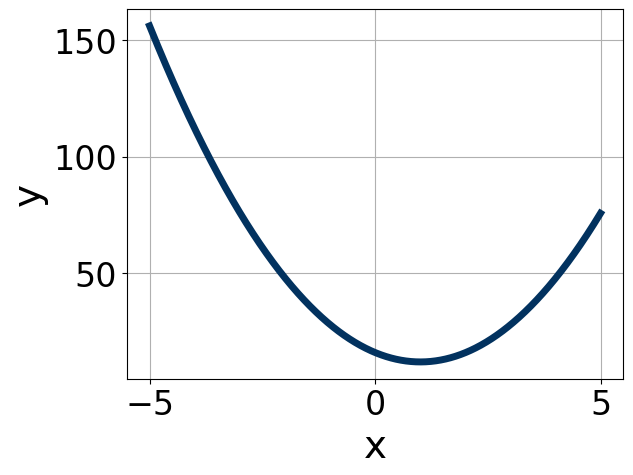
\includegraphics[width = 0.3\textwidth]{../Figures/quadraticEquationToGraphCopyAA.png}\item 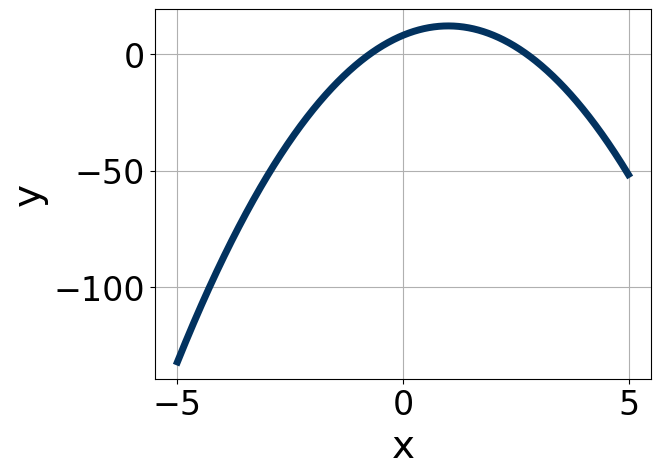
\includegraphics[width = 0.3\textwidth]{../Figures/quadraticEquationToGraphCopyBA.png}\item 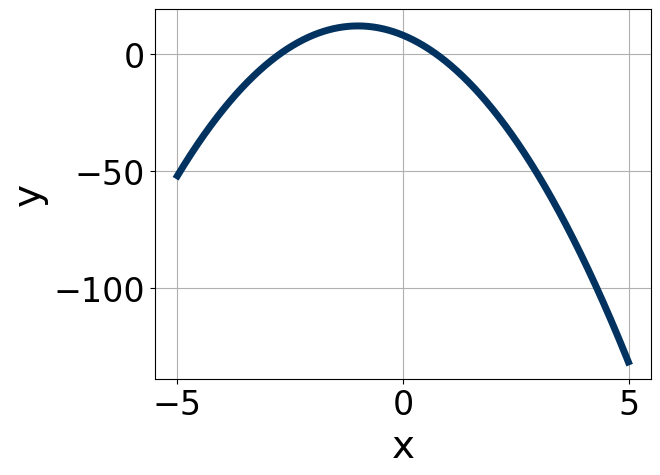
\includegraphics[width = 0.3\textwidth]{../Figures/quadraticEquationToGraphCopyCA.png}\item 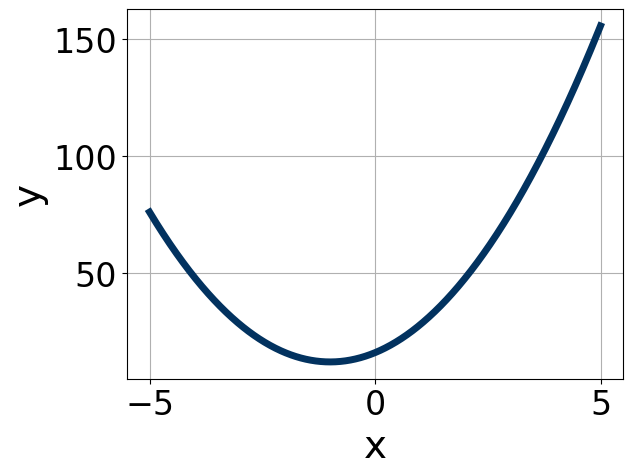
\includegraphics[width = 0.3\textwidth]{../Figures/quadraticEquationToGraphCopyDA.png}\end{multicols}\item None of the above.
\end{enumerate} }
\litem{
Solve the quadratic equation below. Then, choose the intervals that the solutions belong to, with $x_1 \leq x_2$ (if they exist).\[ -12x^{2} -9 x + 2 = 0 \]\begin{enumerate}[label=\Alph*.]
\item \( x_1 \in [-1.22, -0.45] \text{ and } x_2 \in [-0.98, 0.69] \)
\item \( x_1 \in [-14.11, -13.56] \text{ and } x_2 \in [12.66, 13.16] \)
\item \( x_1 \in [-0.3, 0.07] \text{ and } x_2 \in [0.71, 1.12] \)
\item \( x_1 \in [-2.35, -1.93] \text{ and } x_2 \in [10.81, 11.87] \)
\item \( \text{There are no Real solutions.} \)

\end{enumerate} }
\litem{
Factor the quadratic below. Then, choose the intervals that contain the constants in the form $(ax+b)(cx+d); b \leq d.$\[ 16x^{2} -40 x + 25 \]\begin{enumerate}[label=\Alph*.]
\item \( a \in [7.53, 9.57], \hspace*{5mm} b \in [-14, -3], \hspace*{5mm} c \in [1.77, 3.95], \text{ and } \hspace*{5mm} d \in [-8, -4] \)
\item \( a \in [1.91, 3.55], \hspace*{5mm} b \in [-14, -3], \hspace*{5mm} c \in [7.21, 9.2], \text{ and } \hspace*{5mm} d \in [-8, -4] \)
\item \( a \in [3.34, 5.88], \hspace*{5mm} b \in [-14, -3], \hspace*{5mm} c \in [3.86, 4.01], \text{ and } \hspace*{5mm} d \in [-8, -4] \)
\item \( a \in [0.64, 1.35], \hspace*{5mm} b \in [-24, -19], \hspace*{5mm} c \in [0.53, 1.17], \text{ and } \hspace*{5mm} d \in [-23, -16] \)
\item \( \text{None of the above.} \)

\end{enumerate} }
\litem{
Solve the quadratic equation below. Then, choose the intervals that the solutions $x_1$ and $x_2$ belong to, with $x_1 \leq x_2$.\[ 25x^{2} +60 x + 36 = 0 \]\begin{enumerate}[label=\Alph*.]
\item \( x_1 \in [-6.81, -5.76] \text{ and } x_2 \in [-0.36, 0.06] \)
\item \( x_1 \in [-30.51, -28.26] \text{ and } x_2 \in [-30.28, -29.95] \)
\item \( x_1 \in [-3.92, -3.48] \text{ and } x_2 \in [-0.47, -0.38] \)
\item \( x_1 \in [-2.6, -2.14] \text{ and } x_2 \in [-0.95, -0.45] \)
\item \( x_1 \in [-2.12, 0.44] \text{ and } x_2 \in [-1.65, -1.18] \)

\end{enumerate} }
\litem{
Solve the quadratic equation below. Then, choose the intervals that the solutions belong to, with $x_1 \leq x_2$ (if they exist).\[ 19x^{2} +11 x -9 = 0 \]\begin{enumerate}[label=\Alph*.]
\item \( x_1 \in [-20.03, -19.59] \text{ and } x_2 \in [7.1, 8.8] \)
\item \( x_1 \in [-29.09, -27.92] \text{ and } x_2 \in [26.9, 28.8] \)
\item \( x_1 \in [-1.26, -0.72] \text{ and } x_2 \in [-2, 0.9] \)
\item \( x_1 \in [-0.89, -0.22] \text{ and } x_2 \in [0.8, 1.3] \)
\item \( \text{There are no Real solutions.} \)

\end{enumerate} }
\litem{
Graph the equation below.\[ f(x) = (x+3)^2 + 18 \]\begin{enumerate}[label=\Alph*.]
\begin{multicols}{2}\item 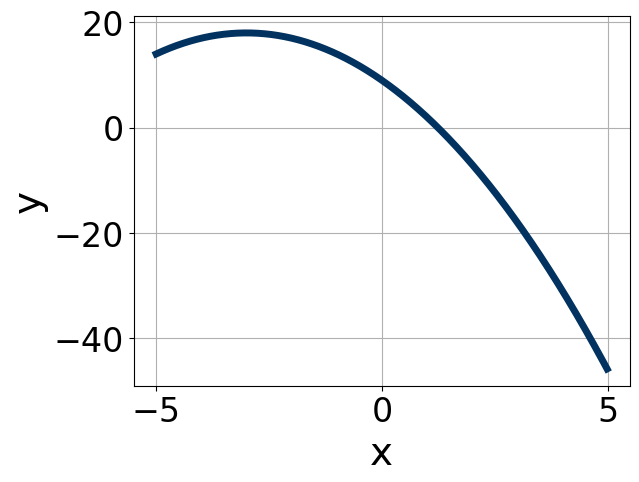
\includegraphics[width = 0.3\textwidth]{../Figures/quadraticEquationToGraphAA.png}\item 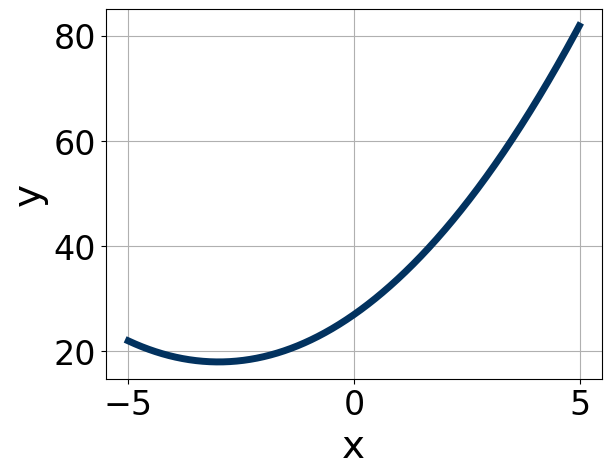
\includegraphics[width = 0.3\textwidth]{../Figures/quadraticEquationToGraphBA.png}\item 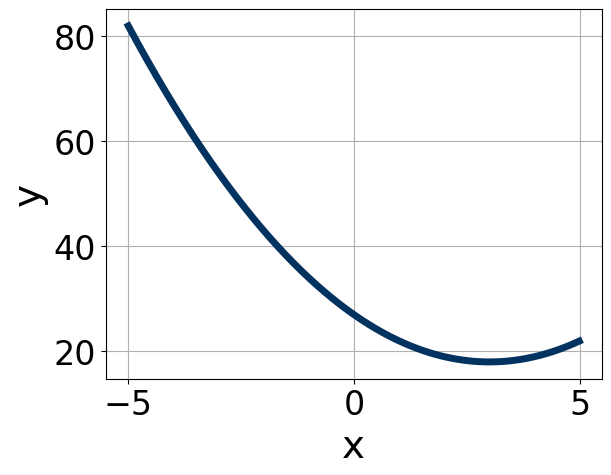
\includegraphics[width = 0.3\textwidth]{../Figures/quadraticEquationToGraphCA.png}\item 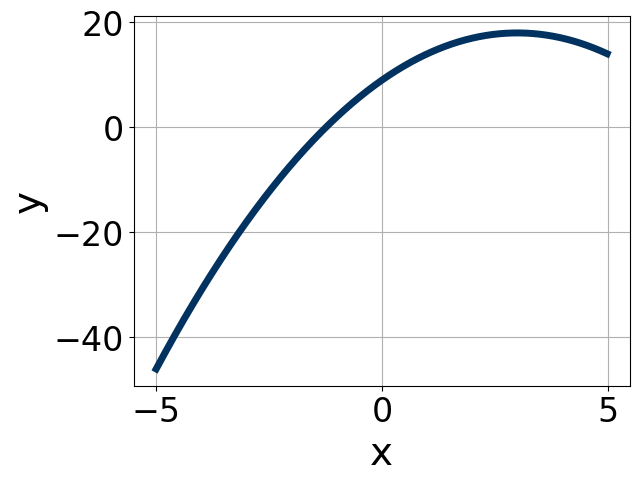
\includegraphics[width = 0.3\textwidth]{../Figures/quadraticEquationToGraphDA.png}\end{multicols}\item None of the above.
\end{enumerate} }
\litem{
Solve the quadratic equation below. Then, choose the intervals that the solutions $x_1$ and $x_2$ belong to, with $x_1 \leq x_2$.\[ 10x^{2} -33 x -54 = 0 \]\begin{enumerate}[label=\Alph*.]
\item \( x_1 \in [-2.15, -1.09] \text{ and } x_2 \in [4.46, 5.37] \)
\item \( x_1 \in [-0.69, -0.37] \text{ and } x_2 \in [12.39, 13.71] \)
\item \( x_1 \in [-2.66, -1.74] \text{ and } x_2 \in [1.04, 3.51] \)
\item \( x_1 \in [-6.77, -5.51] \text{ and } x_2 \in [-1.09, 2.11] \)
\item \( x_1 \in [-12.07, -11.74] \text{ and } x_2 \in [44.34, 46.23] \)

\end{enumerate} }
\litem{
Write the equation of the graph presented below in the form $f(x)=ax^2+bx+c$, assuming  $a=1$ or $a=-1$. Then, choose the intervals that $a, b,$ and $c$ belong to.
\begin{center}
    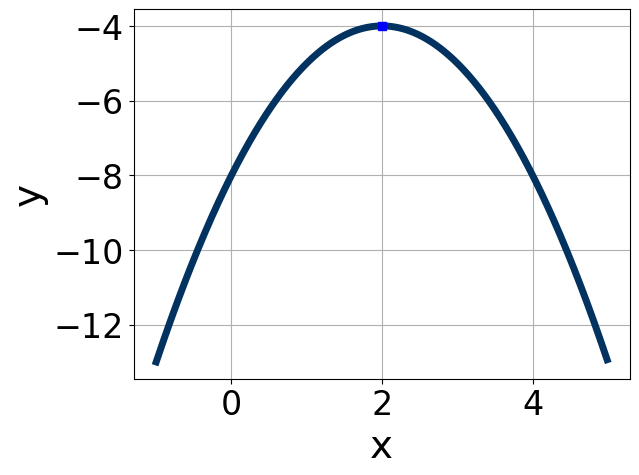
\includegraphics[width=0.5\textwidth]{../Figures/quadraticGraphToEquationA.png}
\end{center}
\begin{enumerate}[label=\Alph*.]
\item \( a \in [1, 2], \hspace*{5mm} b \in [-5, -1], \text{ and } \hspace*{5mm} c \in [-2, 3] \)
\item \( a \in [-3, 0], \hspace*{5mm} b \in [-5, -1], \text{ and } \hspace*{5mm} c \in [-8, -3] \)
\item \( a \in [1, 2], \hspace*{5mm} b \in [3, 6], \text{ and } \hspace*{5mm} c \in [-2, 3] \)
\item \( a \in [-3, 0], \hspace*{5mm} b \in [3, 6], \text{ and } \hspace*{5mm} c \in [-8, -3] \)
\item \( a \in [-3, 0], \hspace*{5mm} b \in [-5, -1], \text{ and } \hspace*{5mm} c \in [-2, 3] \)

\end{enumerate} }
\litem{
Factor the quadratic below. Then, choose the intervals that contain the constants in the form $(ax+b)(cx+d); b \leq d.$\[ 36x^{2} -60 x + 25 \]\begin{enumerate}[label=\Alph*.]
\item \( a \in [3, 5], \hspace*{5mm} b \in [-11, 1], \hspace*{5mm} c \in [11.52, 12.36], \text{ and } \hspace*{5mm} d \in [-9, 1] \)
\item \( a \in [-2, 2], \hspace*{5mm} b \in [-36, -29], \hspace*{5mm} c \in [0.92, 1.31], \text{ and } \hspace*{5mm} d \in [-36, -22] \)
\item \( a \in [9, 19], \hspace*{5mm} b \in [-11, 1], \hspace*{5mm} c \in [2.88, 3.42], \text{ and } \hspace*{5mm} d \in [-9, 1] \)
\item \( a \in [4, 7], \hspace*{5mm} b \in [-11, 1], \hspace*{5mm} c \in [5.85, 6.18], \text{ and } \hspace*{5mm} d \in [-9, 1] \)
\item \( \text{None of the above.} \)

\end{enumerate} }
\litem{
Write the equation of the graph presented below in the form $f(x)=ax^2+bx+c$, assuming  $a=1$ or $a=-1$. Then, choose the intervals that $a, b,$ and $c$ belong to.
\begin{center}
    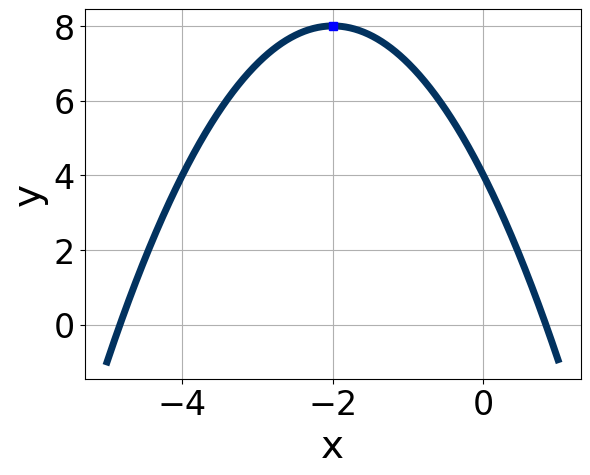
\includegraphics[width=0.5\textwidth]{../Figures/quadraticGraphToEquationCopyA.png}
\end{center}
\begin{enumerate}[label=\Alph*.]
\item \( a \in [1, 2], \hspace*{5mm} b \in [-4, -1], \text{ and } \hspace*{5mm} c \in [10, 15] \)
\item \( a \in [-1, 0], \hspace*{5mm} b \in [-4, -1], \text{ and } \hspace*{5mm} c \in [3, 7] \)
\item \( a \in [1, 2], \hspace*{5mm} b \in [4, 8], \text{ and } \hspace*{5mm} c \in [10, 15] \)
\item \( a \in [-1, 0], \hspace*{5mm} b \in [4, 8], \text{ and } \hspace*{5mm} c \in [3, 7] \)
\item \( a \in [-1, 0], \hspace*{5mm} b \in [4, 8], \text{ and } \hspace*{5mm} c \in [-13, -10] \)

\end{enumerate} }
\end{enumerate}

\end{document}